% !TEX encoding = UTF-8
% !TEX TS-program = pdflatex
% !TEX root = ../tesi.tex

%**************************************************************
\chapter{Il contesto aziendale}

\section{L'azienda}
Siav è una delle più importanti realtà italiane di sviluppo software e di servizi informatici
specializzata nella dematerializzazione e nella gestione documentale e nei processi
digitali. Presenta diverse filiali nel suolo italiano che cooperano tra loro per un fine comune. Siav inoltre punta molto sulla collaborazione tra aziende, in campo nazionale sia a livello pubblico che privato, ma anche a livello internazionale. Una fra tutti Microsoft.
I loro servizi puntano in primo luogo, ad una miglior gestione, controllo ed automazione di tutti i principali processi aziendali; in secondo luogo, ad offrire diverse soluzioni concrete anche a singoli privati che necessitano di sistemi di gestione ed integrazione per lo loro piccola realtà.
\begin{figure}[!h] 
	\centering 
	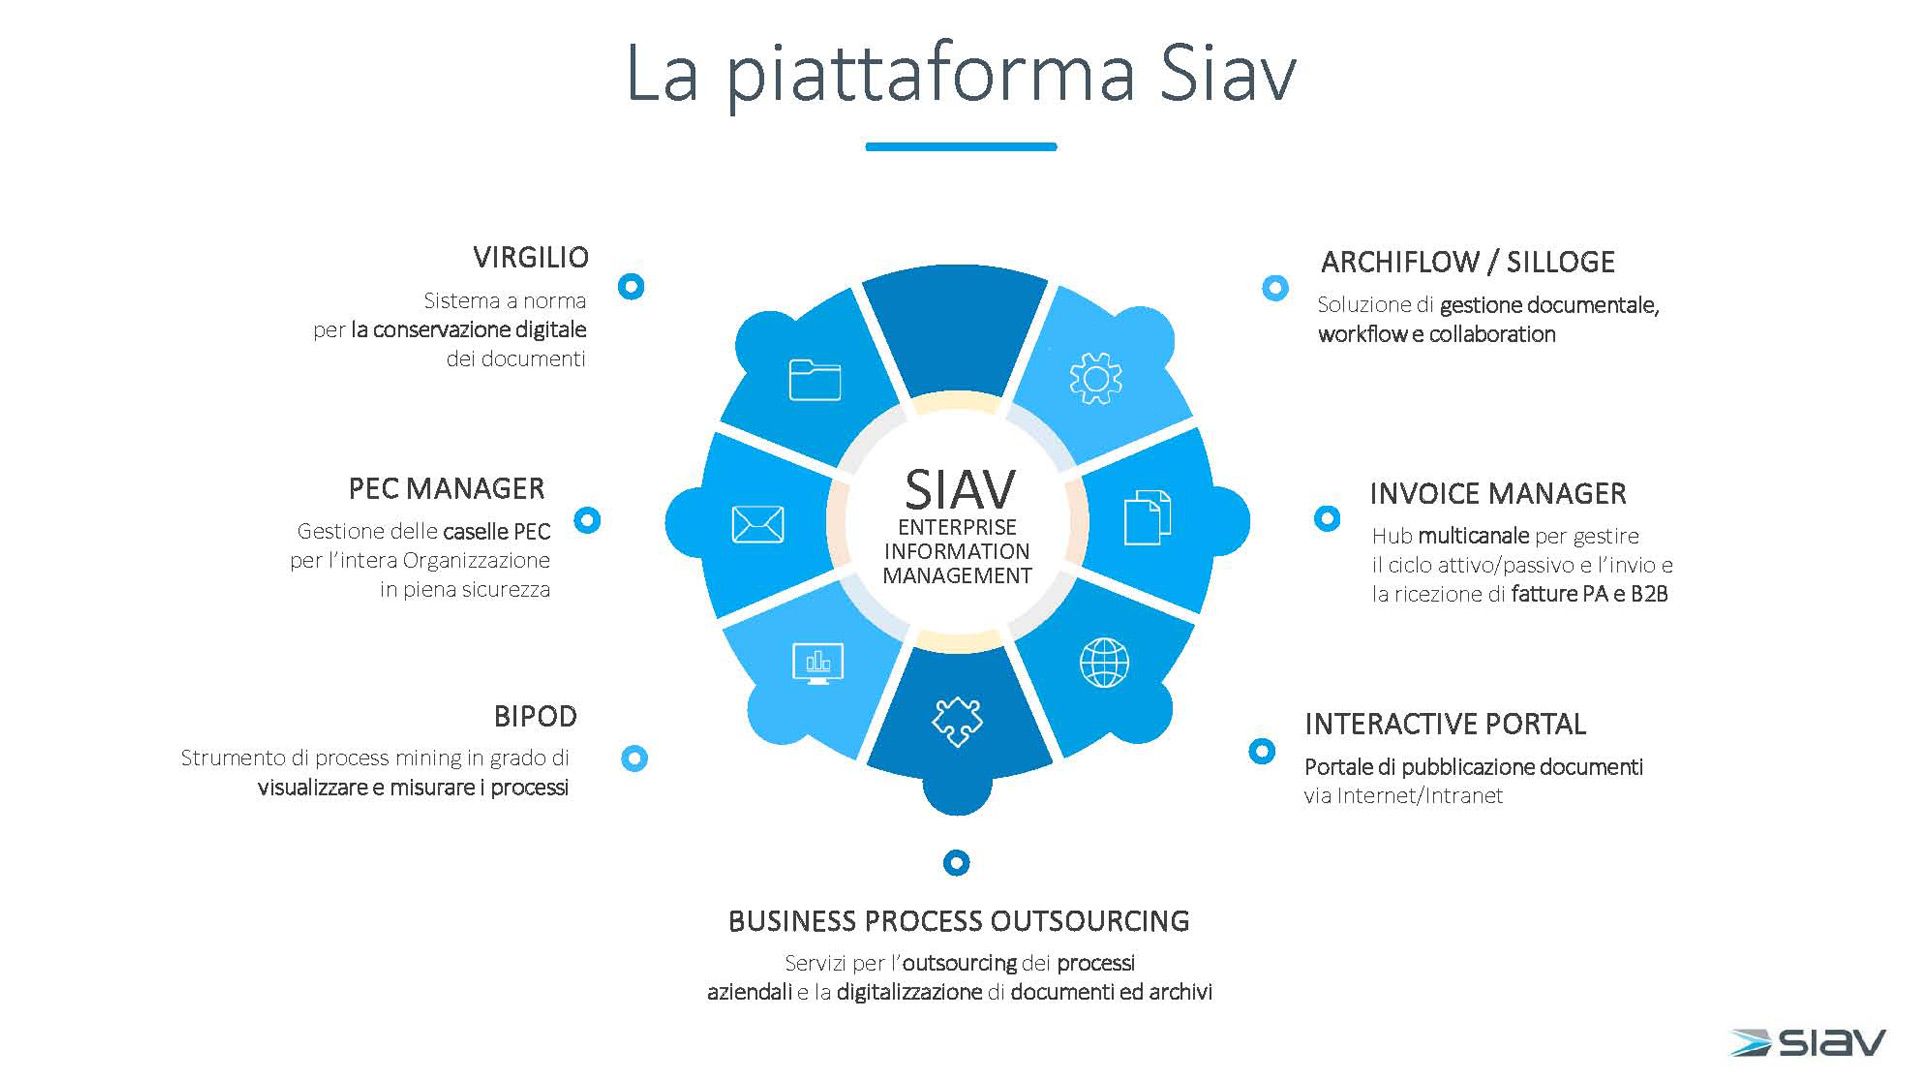
\includegraphics[width=1.1\columnwidth]{siav} 
	\caption{I prodotti offerti da Siav}
\end{figure}
Siav si colloca all'interno del mercato come una tra la più importanti realtà italiane a livello di \textit{Enterprise Content Management} offrendo servizi per poter migliorare processi e gestioni aziendali spaziando da un gestore di caselle PEC, ad un applicativo di process mining denominato \textit{Bipod}, fino ad arrivare al loro prodotto di punta: Archiflow/Silloge: un software in continuo sviluppo, mantenuto e aggiornato da piccoli team che lavorano in sinergia per raggiungere un obiettivo comune. Archiflow/Silloge offre una soluzione alla gestione di una cospicua mole di documenti, categorizzandoli in varie sezioni permettendone un facile reperimento.

\section {Tecnologie utilizzate}
Le tecnologie utilizzate dell'azienda per la realizzazione dei propri prodotti sono fondate principalmente sulla possibilità di un utilizzo tramite cloud. Si sono dedicati principalmente sullo sviluppo di \textit{Webapp}. Tali tecnologie possono essere raggruppate in due macrocategorie: \textit{Frontend} e \textit{Backend}.
\subsection{\textit{Frontend}}
Da quel che ho potuto constatare durante l'attività di stage, per quanto riguarda lo sviluppo web lato \textit{client} viene utilizzata prevalentamente la piattaforma Angular. Tramite il consistente numero di componenti prefabbricati presenti in rete e una vasta gamma di funzionalità e servizi disponibili, è possibile sviluppare un'interfaccia frontend di qualità a proprio piacimento, soddisfando nel miglior modo possibile le aspettative del cliente.

\subsection{\textit{Backend}}
Per quanto riguarda lato backend vengono utilizzate molteplici tecnologie in base alle necessità che prevede il software di sviluppo;  \textit{RabbitMQ}: questa tecnologia è stata pensata principalmente per un'architettura a microservizi e viene utilizzata in più prodotti all'interno dell'azienda. \textit{RabbitMQ} viene definito come un \textit{Broker} di messaggisticia: ossia un sistema che monitora la trasmissioni di messaggi tra servizi.\\ Un'altro sistema utilizzato, restano in ambito di microservizi è \textit{Kubernetes}: un sistema per la gestione di \textit{container}.

\begin{figure}[!h] 
	\centering 
	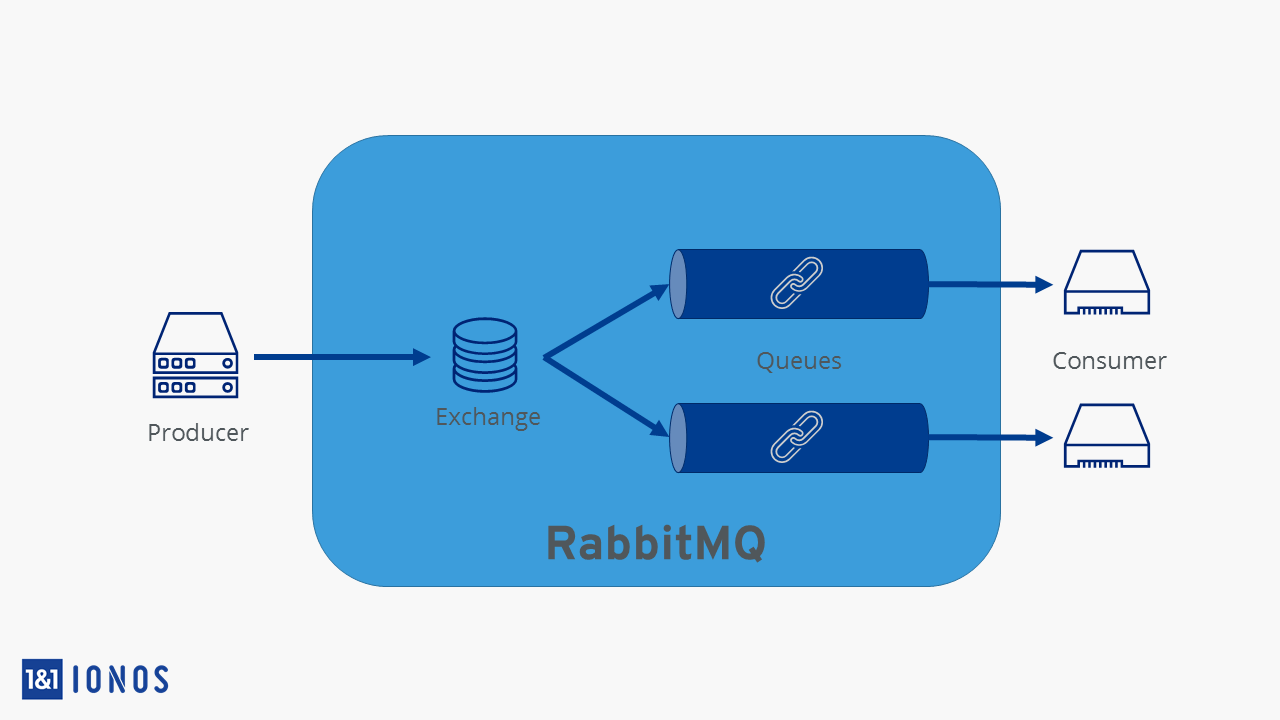
\includegraphics[width=0.8\columnwidth]{rabbitmq} 
	\caption{Diagramm illustrativo sul funzionamento di RabbitMQ}
\end{figure}
\section {Processi aziendali}
\subsection{Metodologie di sviluppo}
L'azienda normalmente si ritrova a dover far fronte ad alcune problematiche derivate da bug, criticità o variazioni importanti di requisiti che possono essere riscontrate durante i vari processi aziendali ed incidere in modo significativo sull'andamento dello sviluppo.
Per cercare di venire incontro a ciò l'azienda ha adottato una metodologia di tipo \textit{Agile}, cercando di mantenere un atteggiamento flessibile rispetto ai processi e gli obiettivi. Risulta quindi fondamentale l'organizzazione di incontri durante vari momenti della giornata o settimana in modo da confrontarsi sull'andamento dei processi e lo stato di avanzamento del prodotto. È consuetudine dei team di lavoro un confronto giornaliero tramite \textit{daily meeting}, per discutere su quanto fatto durante la giornata precedente indicando le eventuali criticità riscontrate, pianificando cosi gli obiettivi per la giornata odierna. Ad inizio settimana invece viene organizzato \textit{weekly meeting} per constatare gli stati di avanzamento rispetto alla settimana precedente, per poi fissare gli obiettivi per la settimana successiva. Gli obiettivi, le attività preposte e le scadenza prefissate venivano solitamente appesi in una lavagna posta in luogo ben visibile all'interno del reparto, per ordine di priorità; in questo modo era quindi possibile tener sott'occhio le principali attività. Il rapporto con il cliente è di vitale importanza per \textit{Siav}. L'azienda infatti presente un servizio di assistenza clienti tramite il quale vengono effettuate segnalazioni di \textit{bug} o assistenza sui proprio prodotti 
\begin{figure}[!h] 
	\centering 
	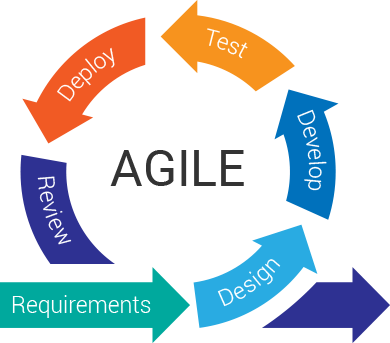
\includegraphics[width=0.4\columnwidth]{agile} 
	\caption{Ciclo di vita della metodologia Agile}
\end{figure}
\subsection{Strumenti di supporto }
L'azienda mette a disposizione diversi strumenti di supporto, allo scopo di gestire e tenere traccia nel migliore dei modi tutte le attività di progetto.
Facendo fede alla metodologia \textit{Agile}, la maggior parte degli strumenti servono a gestire tutti gli aspetti che riguardano il codice. Viene utilizzato \gls{tfs}, uno strumento di \textit{Microsoft} per la gestione delle principali attivtà di progetto che offre un set di strumenti per la collaborazione. Tra le principali funzionalità sono presenti: gestione del repository tramite tecnologie Git o \gls{tfvc}, gestione dei requisiti e strumenti di \textit{build} automatizzati. Tale strumento aderisce in maniera completa a alle tecniche \textit{agile} andando quindi ad integrarsi in modo solido all'interno della realtà lavorativa. Per quanto riguarda il tracciamente delle attività viene utilizzato \textit{Evernote}: un software che permette la scrittura e la condivisione di note all'interno di un gruppo di utenti. Cosi facendo ogni membro del team di sviluppo ha sotto controllo ogni attività svolta dagli altri membri. Un ulteriore strumento utilizzato per il tracciamento dello attività è \textit{Google Docs}. Solitamente i task assegnati presentano una struttura semplice: la data di creazione, la possibilità o meno di menzionare direttamente l'interessato a cui risulta assegnato il task ed un casella di risposta per poter descrivere la sua effettiva terminazione, oppure un messaggio di testo di altro genere, che solitamente indica le problematiche per cui il task non è stato possibile risolverlo. 
\section{Clientela rivolta a Siav}
La maggior parte dei clienti che si affidano a Siav sono aziende che presentano il bisogno di automatizzarsi e migliorare i propri processi interni andando cosi ad incrementare la propria efficenza sotto l'aspetto lavoartivo. Tali aziende sono di vario genere, dal semplice ristorante ad una nota catena di supermercati fino ad aziende metalmeccaniche. Per ogni settore, Siav offre diverse opportunità di gestione e miglioramento aziendale.
Siav è catalogata come \textit{Software house} e presenta un ampio catalogo di prodotti atti a soddisfare le principali necessità organizzative di un'azienda, sta al potenziale cliente poi, valutarne l'acquisto in base alle proprie necessità. 
\subsection{Propensione all'innovazione}
\textit{Siav} è un'azienda che fa dell'innovazione un suo punto cardine. I prodotti che offre sono costantemente aggiornati, cercando di adattarsi alle necessità del cliente. Per poter far ciò l'azienda ha messo a disposizione un serivizio di \textit{Helpdesk} in modo da fornire assistenza in merito ai propri prodotti per i propri clienti. L'azienda inoltre è alla continua ricerca di nuove tecnologie da poter integrare all'interno dei propri applicativi; è presente all'interno dell'organico un team di ricerca e sviluppo che analizza, le varie piattaforme e tecnologie presenti sul mercato. Spesso e volentieri tali attività vengono contestualizzate all'interno di proposte di stage, in modo da poter osservare nel concreto se le ricerche fatte in precedenza possano portare a benefici per i loro prodotti, facendo anche un'attenta analisi dei costi. 